\section{Abläufe und Funktionen}
\label{subsec:szenarien}
\subsection{Anwendungs-Szenarien}
\newcounter{szn}
\setcounter{szn}{1}
\subsubsection*{Szenario \theszn: Pakete erfassen}
Autor: Nha-Dan Tran\\~\\
Es kam gerade eine neue Lieferung an Zutaten und die Pizzabäckerin Antonita muss die angekommenen Waren in das System eingeben. Dafür öffnet sie das Programm und wählt in dem Menü das entsprechende Feld aus. Das Programm bietet ihr an, ein komplett neues Paket anzulegen oder einfach bereits registrierte Pakete aus der Vorlage dem Inventar hinzuzufügen. Da sie auf der Wochenkarte etwas neues ausprobieren wollte, muss sie eine neue Paketvorlage erstellen. Dafür klickt sie auf das entsprechende Feld und es öffnet sich eine Maske, in der sie Farbe, Gewicht, Tragkraft, Breite, Tiefe, Höhe und Unverträglichkeiten eintragen und abspeichern kann.
\stepcounter{szn}
\subsubsection*{Szenario \theszn: Paketvorlagen bearbeiten}
Ein Hersteller hat seine Verpackungsgrößen für Dosentomaten reduziert. Aushilfskraft Karla darf die Änderungen in das System übertragen. Statt 500 g sind nur noch 400 g enthalten und auch die Maße haben sich geändert. Über das Menü des Programms greift sie auf die Vorlagen zu und wählt das zu ändernde Paket aus. Über die Maske kann sie dann Breite, Tiefe, Tragkraft und die Dimension der Vorlage anpassen und abspeichern.
\stepcounter{szn}
\subsubsection*{Szenario \theszn: Pakete anordnen und löschen}
Autor: Aron Schlegel\\~\\
\stepcounter{szn}
Ein Mitarbeiter einer Pizzeria möchte vordefinierte Pakete in ein ebenso vordefiniertes Lagerregal ziehen. Dazu schaut er in dem dafür vorgesehenen Template nach den gewünschten Lebensmittelpaketen, wählt eins aus und zieht es über den gewünschten Platz im Regal. Der Mitarbeiter lässt das Paket los und bekommt eine Fehlermeldung, dass der vorhandene Platz nicht ausreicht und die Tragkraft des Regalbodens überschritten wird. Er beginnt von vorne und lässt das Paket an einer geeigneteren Stelle los, und sieht es nun im Regal stehen. Im Anschluss gefällt ihm die Anordnung eines anderen Paketes nicht. Er möchte dieses lieber auf zwei schon übereinander gestapelte Pakete stellen, Nach dem er das Paket dorthin gezogen hat bekommt er eine Fehlermeldung das die Tragkraft des untersten Pakets nicht ausreichend ist. Er entscheidet sich es am vorherigen Platz stehen zu lassen. 
\subsubsection*{Szenario \theszn: Bestehendes Regal wird umgebaut}
Autor: Aron Schlegel\\~\\
\stepcounter{szn}
Der Mitarbeiter einer Pizzeria möchte ein bereits beladenes Lagerregal umbauen/neu anordnen. Dazu wählt er im System den Regal-Bearbeitungsmodus aus, klickt auf das gewünschte Brett (dieses wird farblich hervorgehoben) und gibt dann die neue Maße und die gewünschte Tragkraft in dem dazu vorgesehenen Eingabefeld ein. Das System prüft daraufhin ob die neuen Konfigurationen im bestehenden Regalsystem Sinn ergeben, und meldet einen Fehler. Die Tragkraft ist nicht ausreichend, für die bereits darauf stehenden Pakete. Daraufhin gibt der Mitarbeiter einen höheren Wert ein, bestätigt und das System akzeptiert. Nachdem das Brett nun neu eingerichtet ist, beendet der Mitarbeiter den Regal-Bearbeitungsmodus. 
\subsubsection*{Szenario \theszn: Regale konfigurieren}
Autor: David Thomann\\~\\
Der Pizzabäcker Anton möchte sein Lager mit unserer Software abbilden. In einem ersten Schritt legt er dafür seine Regale an. Dafür öffnet er sein Lager und nimmt und geht in den Regal-Bearbeitungs-Modus. Im Reitermenü legt er neue Templates für Bretter und Stützen an, mit den Maßen wie er sie auch vor Ort hat, die er mit Drag\&Drop zu einem Nachbau seines echten Regals zusammenbaut. Nachdem er fertig ist, kann er mithilfe eines Häkchens den Regal-Bearbeitungs-Modus verlassen und das System legt sein Regal an. 
\stepcounter{szn}
\subsubsection*{Szenario \theszn: Inventar anzeigen}
Autor: David Thomann\\~\\
Die studentische Aushilfskraft Martin soll einen Abgleich des Lagers mit der Lagerverwaltung machen. Dazu zählt er zuerst die real-existierenden Zutaten im Lager in einer Liste. Danach geht er in die Lager-Verwaltung und öffnet das virtuelle Lager. Über einen Button kann er sich eine aktuelle, nach Zutaten sortierte Auflistung der aktuellen Zutaten anzeigen. Mit dieser Information bringt er das reale Lager und das virtuelle Lager in einem weiteren Schritt wieder auf den selben Stand.
\newpage
\subsection{Anwendungsfälle}
Aus den \hyperref[subsec:szenarien]{\textbf{Anwendungsszenarien}} ergeben sich die folgenden Anwendungsfälle für unsere Software:
\begin{table}[h!]
    % \caption[short]{Tabellarische Auflistung unserer Anwendungsfälle}
    \begin{tabularx}{\textwidth}{l|X}
            \textbf{Ziele / Funktionen} & \textbf{Kurzbeschreibung} \\
            \hline
            Paketvorlage anlegen & Eine Vorlage für ein Paket einer bestimmten Zutat, mit dem dazugehörigen Gewicht, der Tragkraft, den Maßen des Pakets und der Menge an Inhalt anlegen \\
            \hline
            Paketvorlage bearbeiten & Das Gewicht, Tragkraft, Menge oder Maße einer Paketvorlage ändern \\
            \hline
            Pakete erzeugen & Ein Paket aus einem Template erzeugen und platzieren \\
            \hline
            Pakete anordnen & Ein Paket im Regal per Drag\&Drop an einen anderen Ort verschieben \\
            \hline
            Pakete löschen & Ein Paket im Regal löschen \\
            \hline
            Brett- und Stützenvorlage erzeugen & Vorlagen für Bretter und Stützen anlegen \\
            \hline
            Bretter und Stützen erzeugen & Bretter- und Stützenobjekte aus Vorlagen erstellen \\
            \hline
            Bestehende Bretter und Stützen anpassen & Bretter und Stützen die bereits existieren anpassen \\
            \hline
            Bestehende Bretter und Stützen bewegen & Bretter und Stützen im Raum bewegen \\
            \hline
            Regal hinzufügen & In einem leeren Lagerraum ein neues Regal bauen \\
            \hline
            Regal bearbeiten & Ein bereits bestehendes Regal umbauen \\
            \hline
            Inventarliste anzeigen & Zeigt eine nach Zutaten sortierte Liste der in einem Regal vorhandenen Pakete an \\
    \end{tabularx}
\end{table}
\begin{figure}[H]
    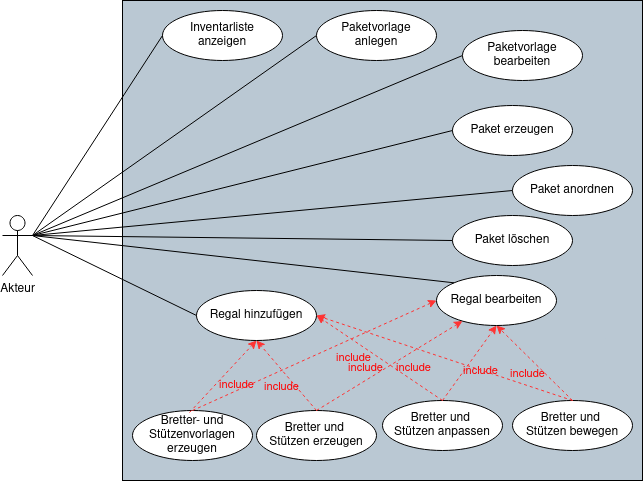
\includegraphics[width=\linewidth]{images/AnwendungsfallDiagramm.png}
    \captionbelow{Anwendungsfall-Diagramm}
    \label{fig:AnwendungsfallDiagramm}
\end{figure}
\clearpage
\subsubsection{Beschreibungen von Anwendungsf\"allen}
\subsubsection*{}
\textbf{Pakete erfassen}\bigskip\\
\textbf{Autor}: Nha Dan-Tran\\
\textbf{Akteure}: Akteur\\
\textbf{Fachlicher Auslöser:} Erfassung der Zutaten im System zur Vorbereitung des effizienten Sortieren\\
\textbf{Vorbedingungen: }-\\
\textbf{Standardablauf:} 

\begin{enumerate}
    \item Akteur: Gibt Art(Bezeichnung), Menge(Anzahl, Int), Farbe(Colourpicker), Gewicht(kg), Tragkraft(kg), Breite x Höhe x Tiefe (cm), Unverträglichkeiten(Liste) ein \label{enum:first}
    \item System: Validiert Eingaben \label{enum:second}
    \item System: Erzeugt Paket und Bestätigen lassen
    \item Akteur: Eingabe bestätigen
    \item System: Legt Paket im Inventar ab.
\end{enumerate}

\textbf{Alternative Abläufe/ Fehlersituationen / Sonderfälle:}
\begin{enumerate}
    \item[] \begin{enumerate}\setcounter{enumi}{1}
        \item Akteur wählt direkt ein bereits existierendes Paket aus und passt lediglich die Menge an
    \end{enumerate}
\end{enumerate}

\begin{enumerate}
    \item[] \begin{enumerate}\setcounter{enumi}{2}
\item System stellt fest, dass es bereits ein Paket mit dieser Bezeichnung gibt und lehnt Erstellung ab
    \begin{enumerate}
    \item System schlägt vor, eine neue Vorlage zu erstellen oder Menge eines bereits existierenden Pakets anzupassen
    \item weiter bei 3
\end{enumerate}
\end{enumerate}
\end{enumerate}

\begin{enumerate}\setcounter{enumi}{2}
\item System lehnt Gewicht oder Dimensionen des Pakets ab, weil sie keinen Sinn ergeben(z.B. 1000 kg oder Maße größer als jegliche Regale). Die entsprechenden Felder werden hervorgehoben
\item Akteur korrigiert betroffene Eingaben
\item weiter bei 3
\end{enumerate}

\textbf{Nachbedingung/Ergebnis:}\\
Inventar wurde aktualisiert und Pakete sind zur weiteren Verteilung im Regalsystem bereit.

\textbf{Nichtfunktionale Anforderungen:\\
}Reaktionszeit \textless 5 Sekunden

\textbf{Parametrisierbarkeit/Flexibilität:}\\
Erstellung von Paketen aus bereits vorhandenen Paketen

\textbf{Nutzungshäufigkeit/Mengengerüst:}\\
Alle 2-3 Tage, je nach 
\par\noindent\rule{\textwidth}{0.4pt}
\subsubsection*{}
\textbf{Paketvorlage bearbeiten}\bigskip\\
\textbf{Autor}: Nha Dan-Tran\\
 \textbf{Akteure}: Chef, Aushilfskraft\\
 \textbf{Fachlicher Auslöser:} Änderungen der Paketgewichte/größe\\
 \textbf{Vorbedingungen: }Pakete sind bereits in der Datenbank angelegt\\
 \textbf{Standardablauf:} 

\begin{enumerate}
    \item Chef/Aushilfskraft wählt zu bearbeitende Vorlage aus dem Inventar aus
    \item Chef/Aushilfskraft ändert entsprechende Felder
    \item System überprüft Eingaben auf Plausibilität
    \item System lässt Eingaben vom Nutzer nbestätigen
    \item Chef/Aushilfskraft bestätigt Eingabe
    \item System aktualisiert die Eingaben in der Datenbank und die Vorlage
\end{enumerate}

\textbf{Alternative Abläufe/ Fehlersituationen / Sonderfälle:}
\begin{enumerate}\setcounter{enumi}{3}
    \item[] \begin{enumerate}
        \item System akzeptiert Eingabe nicht
        \begin{enumerate}
            \item System hebt nicht plausible Eingaben farbig hervor und bittet den Nutzer selbige anzupassen
            \item Nutzer passt Eingaben an
            \item System überprüft Eingaben erneut auf Plausibilität
            \item System akzeptiert Eingaben und lässt den Nutzer bestätigen
            \item Nutzer bestätigt
            \item System aktualisiert Datenbank und Vorlage
        \end{enumerate}
    \end{enumerate}
\end{enumerate}

\noindent\textbf{Nachbedingung/Ergebnis:}\\
Inventar wurde aktualisiert und Pakete sind zur weiteren Verteilung im Regalsystem bereit.

\noindent\textbf{Nichtfunktionale Anforderungen:\\}
Reaktionszeit < 5. sek.

\noindent\textbf{Parametrisierbarkeit/Flexibilität:}\\
Jedes Paket lässt sich somit individuell anpassen.

\noindent\textbf{Nutzungshäufigkeit/Mengengerüst:}\\
Ca. 1 mal im Monat.
\par\noindent\rule{\textwidth}{0.4pt}
\subsubsection*{}
\textbf{Regal anlegen}\bigskip\\
\textbf{Autor}: David Thomann\\
\textbf{Akteure}: Chef, Aushilfskraft\\
\textbf{Fachlicher Auslöser:} Ein neues Regal wurde aufgebaut und soll jetzt im virtuellen Lager erscheinen\\
\textbf{Vorbedingungen: }Lager ist noch nicht voll belegt\\
\textbf{Standardablauf:}
\begin{enumerate}
    \item System: Geht in den Regal-Erstellungs-Modus
    \item Akteur: Erstellt Stützen- und Brettvorlagen, sofern sie noch nicht existieren
    \item Akteur: Zieht Stützen und Bretter aus der Vorlagenliste per Drag\&Drop und ordnet sie entsprechend des echten Regals ans
    \item Akteur: Eingabe bestätigen
    \item System: Legt Regal an
    \item System: Verlässt Regal-Erstellungs-Modus
\end{enumerate}
\textbf{Alternative Abläufe}
\begin{enumerate}
    \item[] \begin{enumerate}\setcounter{enumi}{8}
\item System stellt fest, dass es bereits ein Paket mit dieser Bezeichnung gibt und lehnt Erstellung ab
    \begin{enumerate}
    \item System schlägt vor, eine neue Vorlage zu erstellen oder Menge eines bereits existierenden Pakets anzupassen
    \item weiter bei 3
\end{enumerate}
\end{enumerate}
\end{enumerate}
\textbf{Fehlersituationen:}
\begin{enumerate}
    \item Benutzer wählt Tragkraft für ein Brett, die unter dem Gewicht der aktuellen darauf stehenden Pakete liegt
    \item Benutzer versucht Regal abzuspeichern ohne Stützen am Anfang/Ende des Regals
\end{enumerate}
\textbf{Sonderfälle:}
\begin{enumerate}
\item System lehnt neue Maße für Stützen und Bretter ab, da sie keinen Sinn ergeben (negative Werte, Maße, die nicht ins Lager passen). Der Fehler wird grafisch angezeigt.
\item Akteur korrigiert betroffene Eingaben
\item weiter bei 6
\end{enumerate}
\textbf{Nachbedingung/Ergebnis:}\\
Das System ist wieder im ursprünglichen Modus, das Regal ist mit allen vorher beinhalteten Zutaten in einem neuen Zustand\\
\textbf{Nichtfunktionale Anforderungen:}\\
Plausibitätsfehler werden vom System in max. 200ms angezeigt und können direkt korrigiert werden.\\
\textbf{Parametrisierbarkeit/Flexibilität:}\\
-\\
\textbf{Nutzungshäufigkeit/Mengengerüst:}\\
1-2 mal pro Jahr
\par\noindent\rule{\textwidth}{0.4pt}
\subsubsection*{}
\textbf{Regal bearbeiten}\bigskip\\
\textbf{Autor}: David Thomann\\
\textbf{Akteure}: Chef, Aushilfskraft\\
\textbf{Fachlicher Auslöser:} Ein Regal wurde umgebaut und soll jetzt im Programm angepasst werden\\
\textbf{Vorbedingungen: }System ist im Regal-Bearbeitungsmodus\\
\textbf{Standardablauf:}
\begin{enumerate}
    \item System: Stellt Regal farblich anders dar (Stützen und Bretter) 
    \item Akteur: Wählt Stütze oder Brett aus
    \item Akteur: Passt Stütze und Brett den neuen Maßen und neuer Tragkraft an
    \item System: Prüft neue Maße und neue Tragkraft auf Plausibilität
    \item Akteur: Zieht Stützen und Bretter mittels Drag\&Drop in den real-existierenden Zustand
    \item Akteur: Eingabe bestätigen
    \item System: Eingabe wird geprüft
    \item System: Speichert neue Konfiguration ab
    \item System: Verlässt Regal-Bearbeitungs-Modus
\end{enumerate}
\textbf{Alternative Abläufe}
\begin{enumerate}
    \item[] \begin{enumerate}\setcounter{enumi}{8}
\item System stellt fest, dass es bereits ein Paket mit dieser Bezeichnung gibt und lehnt Erstellung ab
    \begin{enumerate}
    \item System schlägt vor, eine neue Vorlage zu erstellen oder Menge eines bereits existierenden Pakets anzupassen
    \item weiter bei 3
\end{enumerate}
\end{enumerate}
\end{enumerate}
\textbf{Fehlersituationen:}
\begin{enumerate}
    \item Benutzer wählt Tragkraft für ein Brett, die unter dem Gewicht der aktuellen darauf stehenden Pakete liegt
    \item Benutzer versucht Regal abzuspeichern ohne Stützen am Anfang/Ende des Regals
\end{enumerate}
\textbf{Sonderfälle:}
\begin{enumerate}
\item System lehnt neue Maße für Stützen und Bretter ab, da sie keinen Sinn ergeben (negative Werte, Maße, die nicht ins Lager passen). Der Fehler wird grafisch angezeigt.
\item Akteur korrigiert betroffene Eingaben
\item weiter bei 6
\end{enumerate}
\textbf{Nachbedingung/Ergebnis:}\\
Das System ist wieder im ursprünglichen Modus, das Regal ist mit allen vorher beinhalteten Zutaten in einem neuen Zustand\\
\textbf{Nichtfunktionale Anforderungen:}\\
Plausibitätsfehler werden vom System in max. 200ms angezeigt und können direkt korrigiert werden.\\
\textbf{Parametrisierbarkeit/Flexibilität:}\\
-\\
\textbf{Nutzungshäufigkeit/Mengengerüst:}\\
1-2 mal pro Jahr
\par\noindent\rule{\textwidth}{0.4pt}
\subsubsection*{}
\textbf{Pakete im Regal anordnen}\bigskip\\
\textbf{Autor}: Aron-Merlin Schlegel\\
\textbf{Akteure}: Chef, Aushilfskraft\\
\textbf{Fachlicher Auslöser:} Bestellte Lebensmittel sind im Lager einzuräumen \\
\textbf{Vorbedingungen: }Pakete sind erstellt und in Template hinterlegt und Regal ist vollständig konfiguriert.\\
\textbf{Standardablauf:} 
\begin{enumerate}
    \item Mitarbeiter: wählt ein vordefiniertes Template aus und zieht es per Drag \& Drop zur gewünschten Position im Lagerregal.
    \item System: Prüft den ausgewählten Ort auf vier Bedingungen.
    \begin{enumerate}
        \item Tragkraft der darunterliegenden Pakete.
        \item Vorhandener Platz (ausreichend Abstand zu darüberliegender Ablagefläche und Stützen auf linker und/oder auf rechter Seite).
        \item Tragkraft der Ablagefläche.
        \item Unverträglichkeiten zu anderen Lebensmitteln die schon auf dieser Ablagefläche (direkt daneben oder darunter) aufbewahrt werden.
    \end{enumerate}
    \item System: Wenn Bedingungen erfüllt sind, wird das Paket im Regal platziert.
    \item System: Inventarliste wird aktualisiert.
\end{enumerate}
\textbf{Alternative Abläufe/ Fehlersituationen / Sonderfälle:}
\begin{enumerate}
    \item[] \textbf{1a} Mitarbeiter findet kein passendes Template.
    \begin{enumerate}
        \item[] \textbf{1a1} erstellt Template nach Beschreibung.
        \item[] \textbf{1a2} weiter bei 2.
    \end{enumerate}
    \item[] \textbf{3a} Es werden nicht alle vier Bedingungen erfüllt.
    \begin{enumerate}
        \item[] \textbf{3a1} System gibt entsprechende Fehlermeldungen aus.
        \item[] \textbf{3a2} System aktualisiert Inventurliste nicht.
        \item[] \textbf{3a3} Mitarbeiter beginnt wieder bei Punkt 1.
    \end{enumerate}
\end{enumerate}
\textbf{Nachbedingung/Ergebnis:}\\
Paket wird auf Ablagefläche angezeigt und im Inventar gelistet.\\
\textbf{Nichtfunktionale Anforderungen:}\\
Reaktionszeit \textless 5 Sekunden.\\
\textbf{Parametrisierbarkeit/Flexibilität:}\\
-\\
\textbf{Nutzungshäufigkeit/Mengengerüst:}\\
Bis zu mehrmals täglich.
\par\noindent\rule{\textwidth}{0.4pt}
\subsubsection*{}
\textbf{Pakete bewegen und löschen}\bigskip\\
\textbf{Autor}: Aron-Merlin Schlegel\\
\textbf{Akteure}: Chef, Aushilfskraft\\
\textbf{Fachlicher Auslöser:} Lager wird aufgeräumt und alte Packungen aussortiert \\
\textbf{Vorbedingungen: } Pakete sind im Regal aufbewahrt.\\
\textbf{Standardablauf:} 
\begin{enumerate}
    \item Mitarbeiter: Wählt nacheinander Pakete aus, die entsorgt werden sollen und löscht sie
    \item System: Nimmt Paket aus dem Inventar und löscht Paket-Objekt
    \item Mitarbeiter: Zieht nacheinander Pakete per Drag \& Drop an einen neuen Platz
    \item System: Strukturiert Pakete entsprechend in neue Regalabschnitte
    \item Mitarbeiter: Ist fertig
    \item System: Weiterhin betriebsbereit
\end{enumerate}
\textbf{Alternative Abläufe/ Fehlersituationen / Sonderfälle:}
\begin{enumerate}
    \item[] \textbf{2a} Mitarbeiter löscht ein Paket aus Versehen passendes Template.
    \begin{enumerate}
        \item[] \textbf{1a1} System bietet eine Funktion, letzte Aktion rückgängig zu machen
        \item[] \textbf{1a2} weiter bei 2.
    \end{enumerate}
    \item[] \textbf{3a} Mitarbeiter kann alle Pakete aus dem Regal nehmen
    \begin{enumerate}
        \item[] \textbf{3a1} System legt Pakete in temporäre Ablage
        \item[] \textbf{3a2} System geht nicht nicht abgespeicherten Zwischenzustand
        \item[] \textbf{3a3} Mitarbeiter sortiert alles richtig ein und speichert
        \item[] \textbf{3a4} System legt neue Struktur an und geht wieder in Normalzustand
    \end{enumerate}
\end{enumerate}
\textbf{Nachbedingung/Ergebnis:}\\
Regal ist jetzt neu sortiert, keine Nachbedingung - Normaler Zustand\\
\textbf{Nichtfunktionale Anforderungen:}\\
Reaktionszeit \textless 5 Sekunden.\\
\textbf{Parametrisierbarkeit/Flexibilität:}\\
-\\
\textbf{Nutzungshäufigkeit/Mengengerüst:}\\
Circa 1x pro Woche\\
\subsection{Funktionale Anforderungen}
Aus den Anwendungsfällen lassen sich folgende Funktionale Anforderungen an das System ableiten:
\begin{itemize}
  \item Lager muss in Datei verwaltet werden
  \item Regal im Lager muss in Regalteile und Regalabschnitte aufgeteilt sein
  \item Das Regal muss anpassbar bzw. umbaubar sein
  \item Zutaten müssen eine bearbeitbare Auflistung sein
  \item Unverträglichkeiten zwischen Zutaten müssen eingestellt werden können
  \item Templates müssen verwaltet erstellt werden können
  \item Alle Aspekte der Templates müssen anpassbar sein
  \item Pakete müssen dem Regal hinzugefügt und gelöscht werden können
  \item Pakete müssen gestapelt werden können
  \item Pakete müssen umsortiert werden können, der Regalabschnitt in dem sie sich befinden, muss ermittelt werden können
\end{itemize}
\subsection{Nicht-Funktionale Anforderungen}
\textbf{Zuverlässigkeit und Verfügbarkeit:}
\begin{itemize}
  \item Das System sollte lokal auf den Rechnern der Pizzeria laufen
  \item Daten müssen zuverlässig und persistent gehalten werden
\end{itemize}
\textbf{Leistung und Skalierbarkeit:}
\begin{itemize}
  \item Drag\&Drop-Vorgänge müssen flüssig ablaufen und Fehlerzustände schnell erkannt und angezeigt werden (\textless 200ms) 
  \item Es sollte möglich sein, mehrere Lager zu erfassen
\end{itemize}
\textbf{Benutzerfreundlichkeit:}
\begin{itemize}
  \item Die GUI sollte ohne Fachwissen und Schulung zu bedienen sein (Buttons \& farbliche Hervorhebung von Interaktionspunkten) 
  \item Es sollte möglich sein, das System auf mehreren Geräteklassen nutzen zu können
\end{itemize}